\documentclass[../main.tex]{subfiles}
\begin{document}

\chapter{Annex}

\section{Annex for Chapter 2}
\label{app:background_work}

\section{Annex for Chapter 3}
\label{app:avatar_creation_pose_synthesis}

\section{Annex for Chapter 4}
\label{app:multi_track}

\section{Annex for Chapter 5}
\label{app:intermediate_blocks_pose_correction}

\subsection{AZee Rules Frequency}
\label{app:intermediate_blocks_pose_correction:azee_rules_frequency}

\begin{figure}[h]
    \centering
    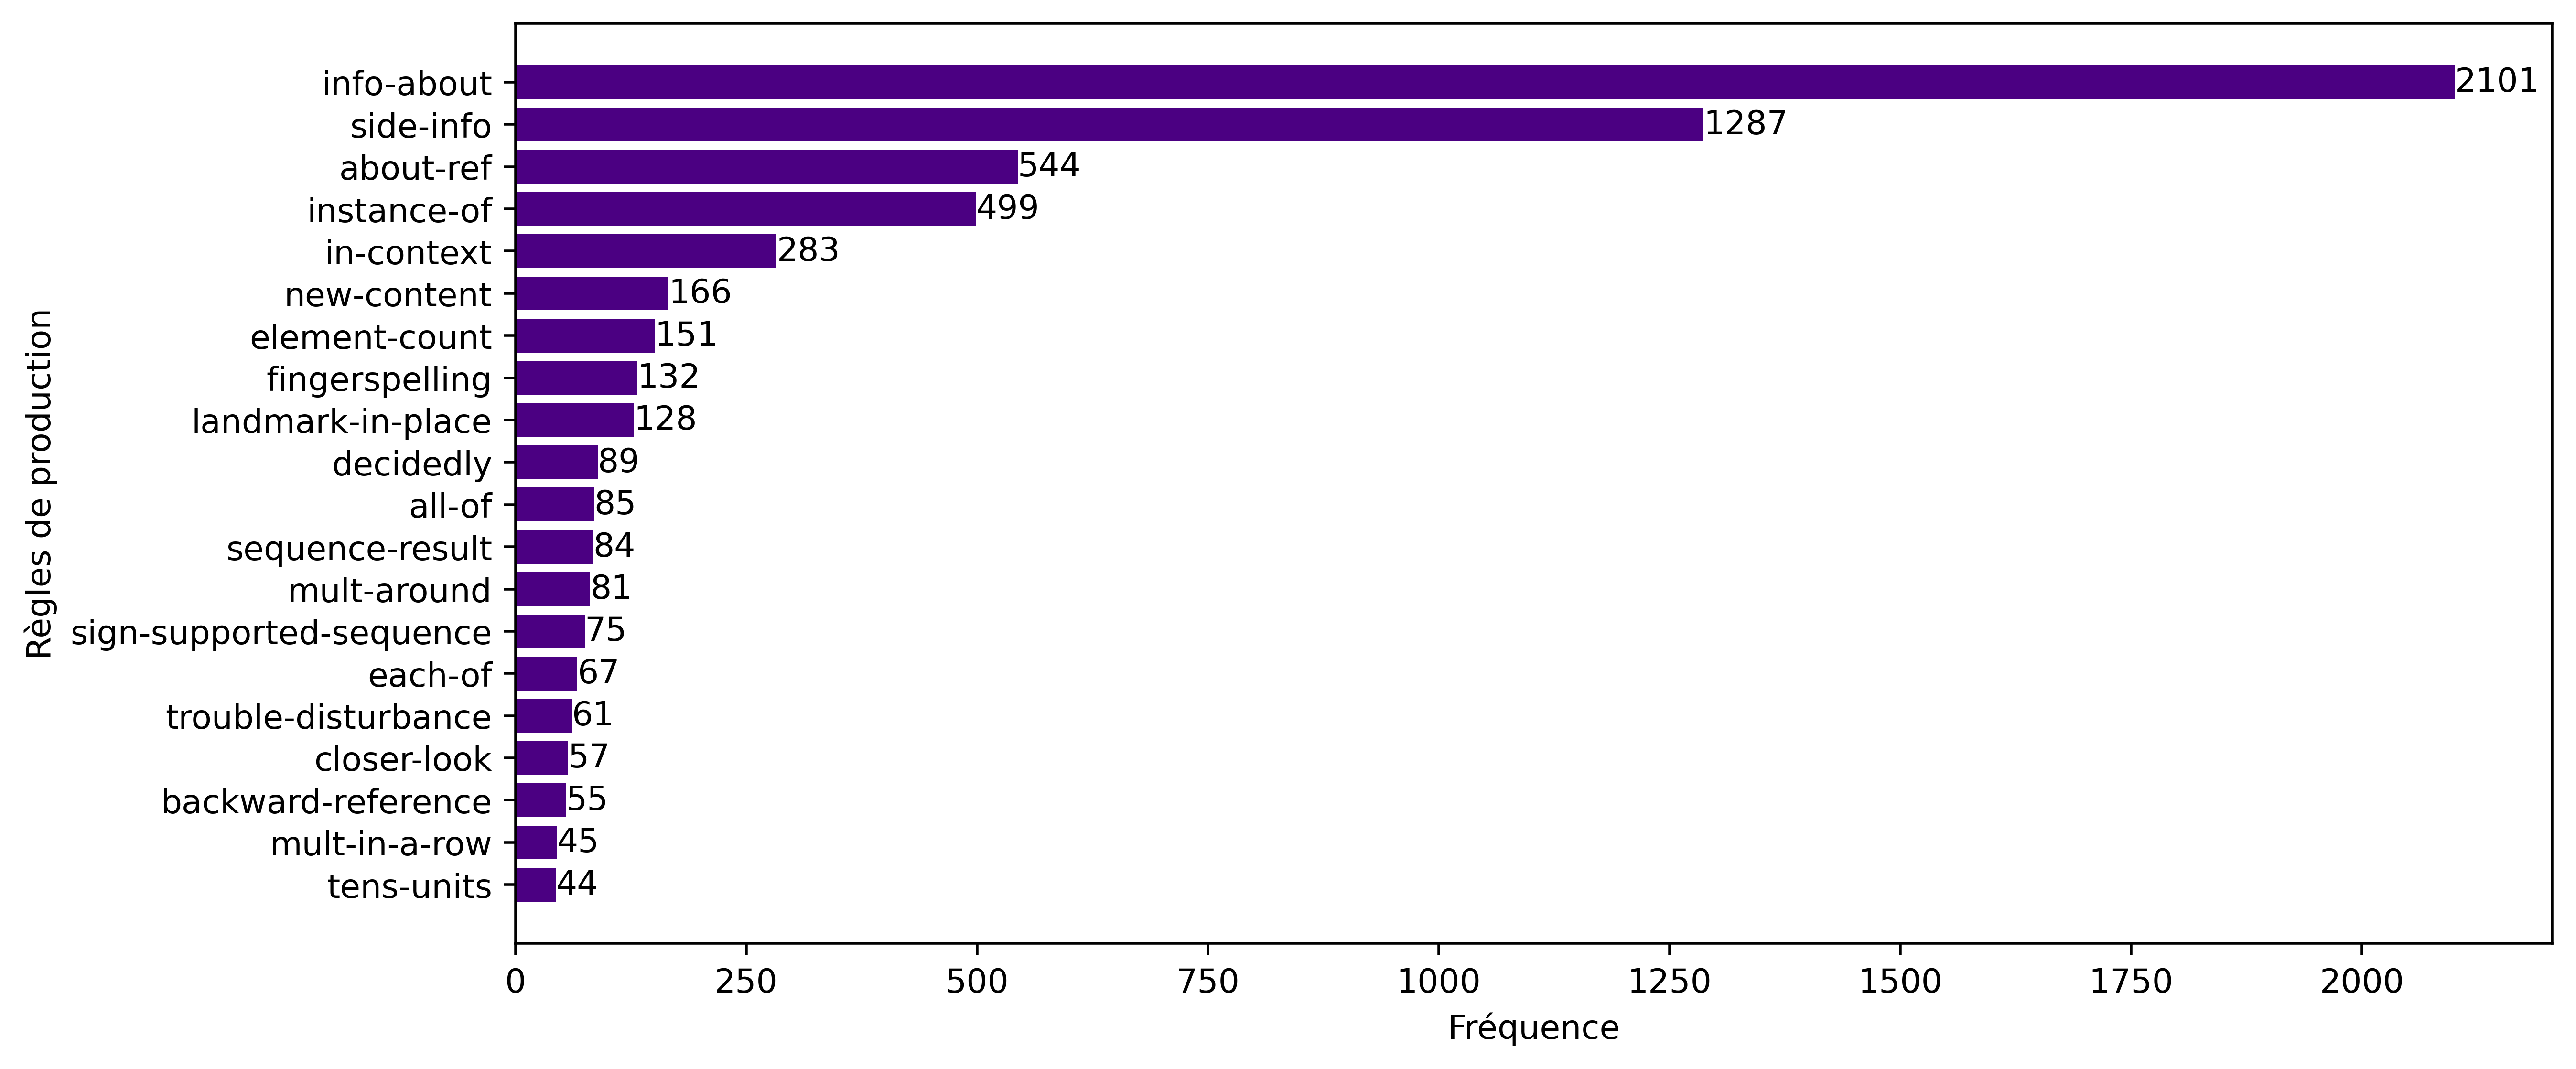
\includegraphics[width=5in]{chapters/intermediate_blocks_pose_correction/images/azee_rule_frequency.png}
    \caption{Frequency of AZee rules in the \emph{40 brèves} corpus}
    \label{fig:azee_rule_frequency_ch1}
\end{figure}

\subsection{Pose Estimation based templates}
\label{app:intermediate_blocks_pose_correction:pose_est_templates}

In future, the procedurally generated templates can also be based on the AZee rule and corresponding motion data based on motion curves from videos directly using pose estimation techniques~\ref{fig:motion_curves_template_procedural_pose_est}.

\begin{figure}
    \centering 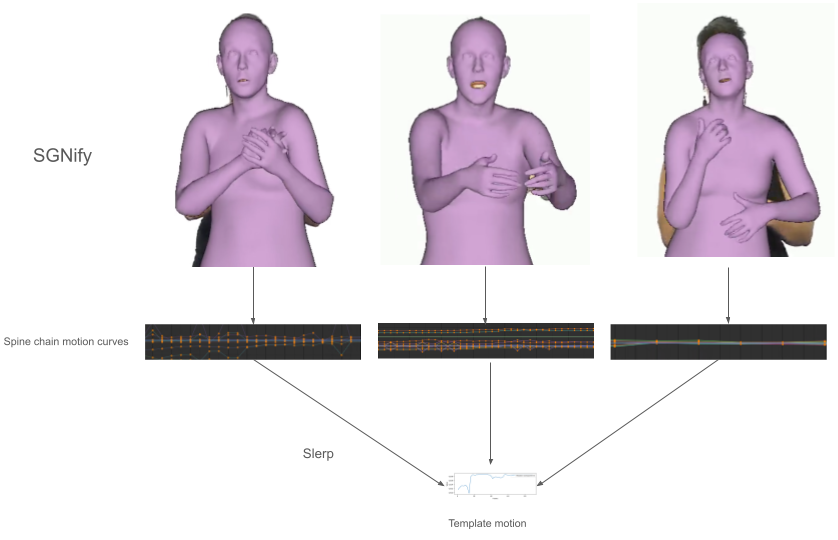
\includegraphics[width = 5in]{chapters/intermediate_blocks_pose_correction/images/motion_curves_template_procedural_pose_est.png}
    \caption{Procedurally Generated motion curves for template \emph{info-about}}
    \label{fig:motion_curves_template_procedural_pose_est}
\end{figure}

\section{Annex for Chapter 6}
\label{app:facial_expressions}

\subsection{Facial expressions using FLAME}
\label{app:facial_expressions:flame}

\begin{longtable}{|l|c|r|}
    \caption{Synthesized Expressions} \label{tab:facial_expressions} \\
    \hline
    \textbf{AZee rule} & \textbf{Original Expression} & \textbf{FLAME}  \\
    \hline
    \endfirsthead

    \hline
    \textbf{AZee rule} & \textbf{Original Expression} & \textbf{FLAME} \\
    \hline
    \endhead

    \hline
    \endfoot

    \hline
    \endlastfoot

    \emph{big-threatening} & \includegraphics[width=0.15\textwidth]{chapters/facial_expressions/images/original_facial_expressions/big_threatening.png} & \includegraphics[width=0.15\textwidth]{chapters/facial_expressions/images/flame_facial_exps/big_threatening.png} \\
    \emph{continuously} & \includegraphics[width=0.15\textwidth]{chapters/facial_expressions/images/original_facial_expressions/continuously.png} & \includegraphics[width=0.15\textwidth]{chapters/facial_expressions/images/flame_facial_exps/continuously.png} \\
    \emph{do-you-realise} & \includegraphics[width=0.15\textwidth]{chapters/facial_expressions/images/original_facial_expressions/do_you_realise.png} & \includegraphics[width=0.15\textwidth]{chapters/facial_expressions/images/flame_facial_exps/do_you_realise.png} \\
    \emph{it-is-a-shame} & \includegraphics[width=0.15\textwidth]{chapters/facial_expressions/images/original_facial_expressions/it_is_a_shame.png} & \includegraphics[width=0.15\textwidth]{chapters/facial_expressions/images/flame_facial_exps/it_is_a_shame.png} \\
    \emph{uneasy-awkward} & \includegraphics[width=0.15\textwidth]{chapters/facial_expressions/images/original_facial_expressions/uneasy_awkward.png} & \includegraphics[width=0.15\textwidth]{chapters/facial_expressions/images/flame_facial_exps/uneasy_awkward.png} \\
    \emph{with-no-precision} & \includegraphics[width=0.15\textwidth]{chapters/facial_expressions/images/original_facial_expressions/with_no_precision.png} & \includegraphics[width=0.15\textwidth]{chapters/facial_expressions/images/flame_facial_exps/with_no_precision.png} \\
    \emph{with-surprise} & \includegraphics[width=0.15\textwidth]{chapters/facial_expressions/images/original_facial_expressions/with_surprise.png} & \includegraphics[width=0.15\textwidth]{chapters/facial_expressions/images/flame_facial_exps/with_surprise.png} \\
    \emph{with-uncertainty} & 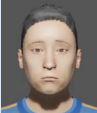
\includegraphics[width=0.15\textwidth]{chapters/facial_expressions/images/original_facial_expressions/with_uncertainty.png} & 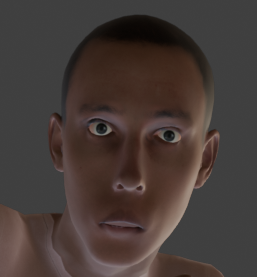
\includegraphics[width=0.15\textwidth]{chapters/facial_expressions/images/flame_facial_exps/with_uncertainity.png} \\
    \emph{with-worry} & \includegraphics[width=0.15\textwidth]{chapters/facial_expressions/images/original_facial_expressions/with_worry.png} & \includegraphics[width=0.15\textwidth]{chapters/facial_expressions/images/flame_facial_exps/with_worry.png} \\
\end{longtable}

\end{document}
